\chapter{Detalles de Implementación y Experimentos}\label{chapter:implementation}
La aplicación resultante de esta investigación está implementada en Visual Code, en Python 3.11.5
debido a la experiencia en el lenguaje y a la no especificación de requerimientos de programación. Cabe 
recalcar que el diseño del proyecto se puede realizar en casi cualquier lenguaje y plataforma. \nocite{Aguilar2010}

\section{Detalles de Implementación}
El proyecto se encuentra dividido en varios módulos que se pueden representar en dos secciones.
La primera sería la sección de la lógica del proyecto, en esta se encuentran los módulos dedicados 
a la lógica de los agentes, la creación del entorno\footnote{Grafo de localizaciones y de relaciones}
y un último que es el encargado de realizar las simulaciones. La segunda sección es la encargada de 
la parte visual del proyecto, posee un único módulo denominado $frontend$\footnote{Termino utilizado en 
Ingeniería de Software para referirse a la parte visual de un aplicación} el cual es el designado para permitirle
al usuario interactuar con la aplicación; es decir, introducir las variables del modelo, simular, 
graficar los resultados obtenidos, entre otras acciones.

El conocimiento de la complejidad temporal del modelo generado permite entender la mejor manera de usarlo.
Esta complejidad temporal está dada por:
\begin{center}
    Sea $h$ la cantidad de horas a simular.\\
    Sea $p$ la cantidad de personas incluidas en la simulación.\\
    Sea $m_l$ la cantidad de mosquitos por localizaciones escogidos para picar en esa hora.\\
    Entonces la complejidad temporal del modelo es $O(h \times p \lbrack 3 \times 13 \times 16 + 14 + m_l \rbrack)$
\end{center}

Es fácil apreciar que si $h = p$ en nuestra simulación, entonces la complejidad pasaría a ser cuadrática, ya 
que sería $p^2$. En el caso de que $m_l = p$, sería cuadrática también, pero $m_l$ es un valor 
que depende de una probabilidad por lo tanto el modelo no siempre procesaría el conjunto de mosquitos completos,
por lo que, para el peor caso\footnote{Peor caso: siempre se escogen todos los mosquitos del lugar para que piquen} demoraría
lo mismo, pero por lo general, sería más rápido.



\section{Experimentación}
Para la validación del modelo implementado se hizo necesario generar varios grafos con distintos parámetros.
En \autocite{Arazoza2010} se proponen unos valores fijos para ciertas variables de interés de este proyecto.\\

\textbf{Datos de estimaciones anteriores:}\autocite{Arazoza2010}
\begin{itemize}
    \item Tasa de mortalidad de humanos (0.000024).
    \item Tasa de recuperación de la enfermedad (0.143).
    \item Tasa de transmisión de humano a mosquito (entre 0.16346 y 0.16384).
\end{itemize}

La correcta evolución del modelo propuesto depende en gran medida de los valores de los parámetros que lo  
caracterizan y que, en su mayoría, se han considerado como constantes\footnote{Constantes para una 
instancia de simulación, pues pueden variar de una a otra}. La obtención de valores 
adecuados para estos parámetros es esencial para garantizar que el modelo refleje con precisión el 
fenómeno que se está estudiando. Para lograrlo, se requiere la contribución de expertos en áreas específicas 
de la ciencia que posean conocimientos y experiencia en la caracterización y medición de los parámetros.
Para grafos semejantes o isomorfos el modelo no necesariamente brinda resultados parecidos. Esto no solo 
se debe a la estocasticidad con la que se define el mismo, puede producirse también por valores de 
parámetros distintos; pero, grafos semejantes, con valores iguales de parámetros brindarían 
resultados muy parecidos. Con la idea de reflejar esto se realizaron simulaciones con valores distintos
para cada variable en cuestión.

Una idea seguida en la validación se basa en el concepto de $self-averaging$\footnote{auto-promediado} que se refiere a la propiedad de 
ciertas cantidades físicas en un sistema que exhiben una consistencia y estabilidad estadística a medida 
que el tamaño del sistema se vuelve grande. \

Cuando una cantidad física es auto-promediada, significa que su valor promedio se puede 
obtener a partir de una única realización del sistema, y que el promedio sobre múltiples 
realizaciones del sistema no introduce una variabilidad significativa en el valor promedio. 
En otras palabras, si se toman diferentes muestras del sistema y se calcula el promedio de 
la cantidad de interés en cada una de ellas, los valores promedio obtenidos serán 
consistentes y estarán cerca del valor promedio obtenido a partir de una sola muestra.

El concepto de auto-promediado es útil porque simplifica el análisis de sistemas físicos. 
Si una cantidad es auto-promediada, entonces es suficiente estudiar un único sistema grande 
para obtener información precisa sobre el comportamiento promedio del sistema en general. 
Esto es especialmente importante en sistemas complejos, donde realizar múltiples simulaciones 
o experimentos puede ser costoso o difícil.

% Una idea seguida para la experimentación se basa en:
% \begin{center}
%     Sean $G_1=(V_1, E_1)$ y $G_2=(V_2, E_2)$ grafos de la simulación.\\
%     $V_1 > V_2$ y $E_1 > E_2$.\\
%     Sea $C_1$, $C_2$ la conectividad de $G_1$, $G_2$ respectivamente.\\
%     Si $C_1 = C_2$ se podría decir que estos grafos describen el mismo problema, es decir
%     la curva de infección de $G_1$ sería similar a la de $G_2$.
% \end{center} 



% Por como se modeló el proyecto no solo influye el grado de conectividad para la infección o no de las personas,
% también influyen las acciones que realizan y la estocasticidad debido a los parámetros de 
% infección\footnote{Probabilidad de picar y Probabilidad de infectarse}, pero dejando a un lado estos dos 
% últimos puntos se puede afirmar que se cumple la implicación anterior.

% Debido a esto se entiende que es suficiente simular el proceso con una cantidad considerable de personas,
% pero no es necesario hacerlo para el número exacto que se quiere simular. Por ejemplo,
% si se desea simular para $p = 1000000$\footnote{$p$ cantidad de personas} en caso de que para $p = 1000$ 
% se encontrara un grado de conectividad similar al del primer grafo, entonces la curva de infección
% de este segundo, describiría la del primero. Sin embargo, si se cuenta 
% con el tiempo necesario, podría ser útil hacerlo para el número de personas que se quiera. 

En la siguiente gráfica se muestra como varían los valores de los conceptos referentes a las acciones
cuando solo existe una persona en la simulación.

\begin{figure}[htb]
    \centering
    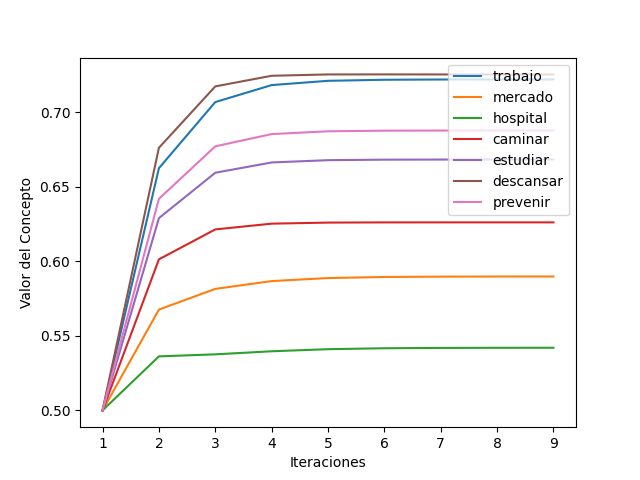
\includegraphics[width=0.9\textwidth]{Graphics/Conceptos_Valores_Normales.png}
    \caption{Valores de los Conceptos de Acciones para nueve iteraciones de una persona}
\end{figure}

Se puede apreciar en la figura 3.1 como en la primera iteración todos los conceptos tienen valor
igual a $0.5$ esto se debe a que en la 1ra instancia los valores referentes a los conceptos
de sentimiento son $0$ por lo tanto, la función sigmoidal devuelve $0.5$.

Como se observa en la figura, a partir de la tercera iteración todos los conceptos varían 
muy poco su valor, es por lo cual se decidió, que cada vez que una persona fuese a realizar
una acción, se ejecutaran tres actualizaciones del $FCM$. La primera para obtener la percepción
que tiene en el momento, la segunda para actualizar los pesos de sentimientos y acciones con
respecto a esa percepción y la tercera para estabilizarlos. Con esta idea
se logra efectuar una acción en dependencia de cómo se sienta el humano en cuestión.

Es importante recalcar que esta figura también demuestra que el $FCM$ funciona de acuerdo a lo 
que se quería modelar. Las acciones de $trabajar$ y $descansar$ son las que más se ejecutarían
en un entorno individual, ambas con valores muy parecidos.

Otro aspecto a notar del gráfico es que la acción de $ir$ $al$ $hospital$ es poco probable que 
se ejecute si la persona no se encuentra enferma, esto con la misma intención de representar la 
realidad. Sin embargo los pesos, como se explicó, cambian de acuerdo a lo que sucede, por tanto,
en algunos momentos de la simulación, si se presentan las condiciones, ir al trabajo,
podría ser la acción que menos peso tuviera.

Para validar los resultados que retorna el modelo se simuló $30$ veces con los parámetros a continuación:
\begin{itemize}
    \item Cantidad de personas: 1000
    \item Cantidad de Días: 365
    \item Valor del Mercado: 250
    \item Probabilidad de aristas: 0.07
    \item Cantidad de Mosquitos por lugares: 40
    \item Probabilidad de Picar: 0.02
    \item Probabilidad de Infectarse: 0.15
    \item Probabilidad de Morir: 0.000024
    \item Trabajos: 2
    \item Mercados: 1
    \item Hospitales: 1
\end{itemize}
\vspace{0.50cm}

\textbf{Estadística de las simulaciones:}
\begin{itemize}
    \item Promedio de personas infectadas: 534
    \item Desviación estándar: 39
    \item Por ciento que representa la desviación estándar con respecto al promedio de personas infectadas: 7.3\%
\end{itemize}

Por estos datos reflejados se entiende que el sistema en relación
a la cantidad de personas infectadas es auto-promediado, pues el hecho de que una desviación estándar represente aproximadamente el 7\% 
del valor promedio sugiere que la variabilidad entre las realizaciones del sistema es relativamente baja en comparación con el valor 
promedio. Esto indica una cierta consistencia y estabilidad estadística en las simulaciones. A partir de esto, para cualquier valor 
de personas mayor a $1000$ basta con simular una sola vez.\\


\begin{figure}[htbp]
    \centering
    \begin{minipage}[t]{0.50\textwidth}
    \centering
    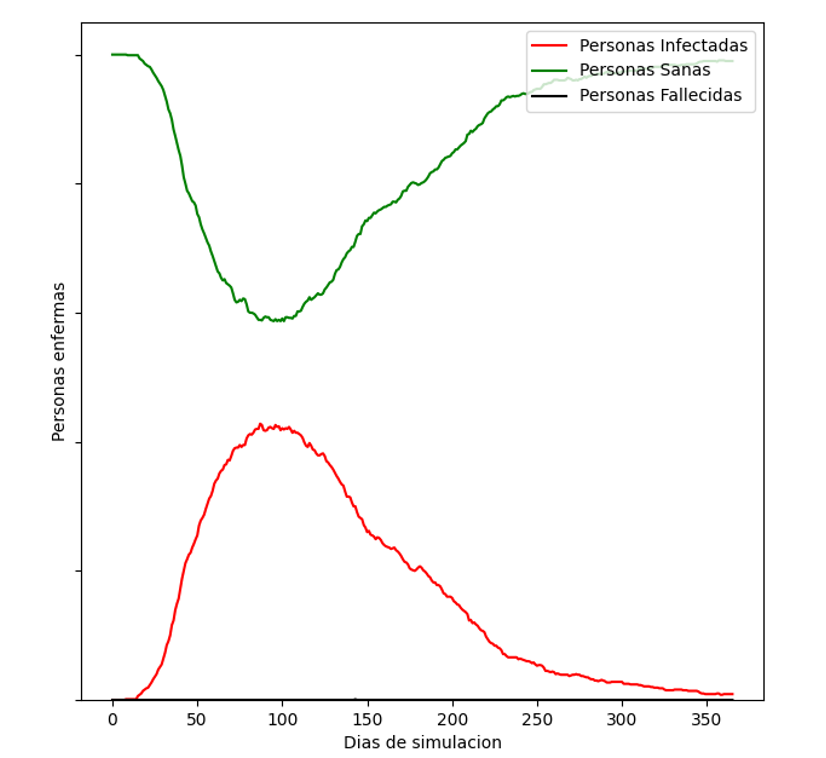
\includegraphics[width=\textwidth]{Graphics/I_M_S_1000.png}
    \caption{Gráfica de la simulación}
    \end{minipage}\hfill
    \begin{minipage}[t]{0.50\textwidth}
    \centering
    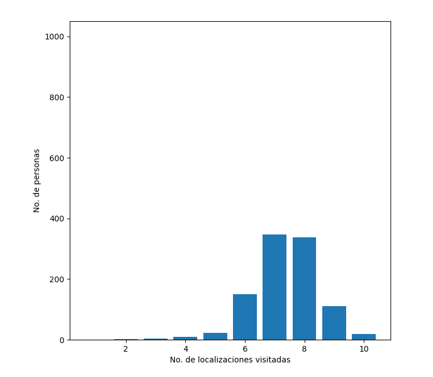
\includegraphics[width=\textwidth]{Graphics/Loc_Vist_1000.png}
    \caption{Cantidad de personas que visitaron $x$ localizaciones}
    \end{minipage}
\end{figure}

\begin{figure}[htb]
    \centering
    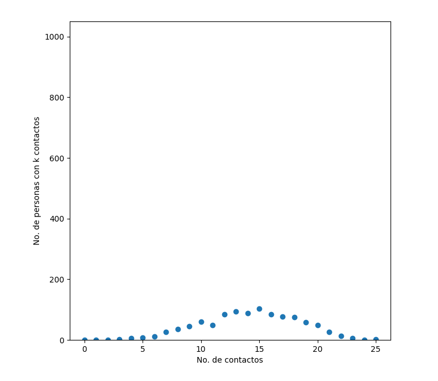
\includegraphics[width=0.55\textwidth]{Graphics/Contactos_Pers_1000.png}
    \caption{Cantidad de personas con $k$ contactos}
\end{figure}

Los gráficos representan un ejemplo de una simulación para 1000 personas.
\newpage
Comparando con los resultados obtenidos por \autocite{Arazoza2010}:
\begin{figure}[htbp]
    \centering
    \begin{minipage}[t]{0.50\textwidth}
    \centering
    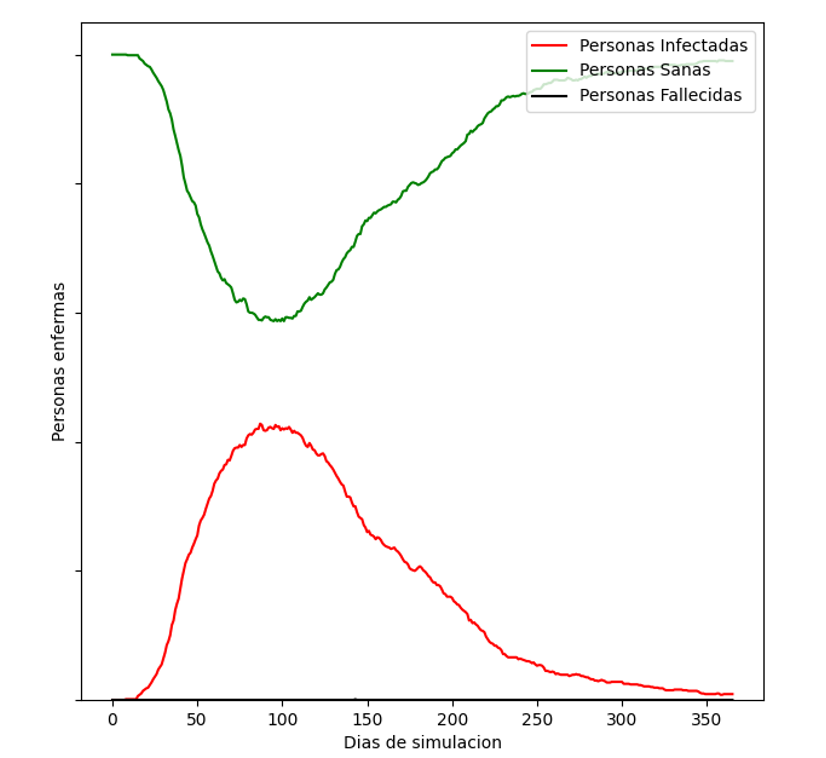
\includegraphics[width=\textwidth]{Graphics/I_M_S_1000.png}
    \caption{Datos y estimaciones de humanos infectados del modelo (1000)}
    \end{minipage}\hfill
    \begin{minipage}[t]{0.50\textwidth}
    \centering
    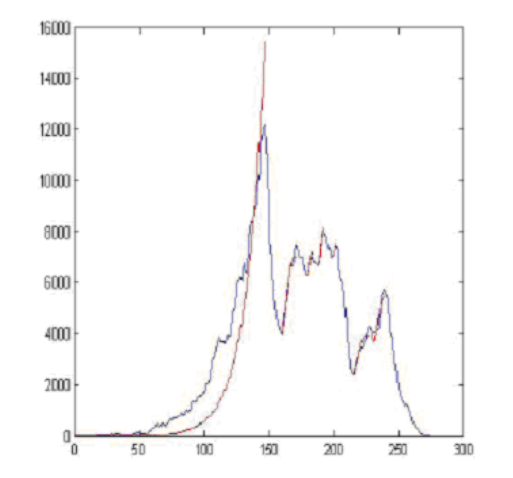
\includegraphics[width=\textwidth]{Graphics/Aymee_Esti.png}
    \caption{Datos y estimaciones de humanos infectados \autocite{Arazoza2010}}
    \end{minipage}
\end{figure}

La curva azul representa a los datos y la roja a las estimaciones en la figura derecha. 
Los descensos que se aprecian son debidos a las campañas de fumigación,
es un efecto externo que nuestra simulación no tiene en cuenta, ya que los agentes son los encargados
de protegerse, por lo que en esta solo existe un descenso. A pesar de las diferencias entre parámetros
como la cantidad de personas, se observa que ambos resultados alcanzan el pico de la epidemia entre los 
$100$ y $150$ días de simulación.

Como validación final del modelo implementado se realizó una simulación de $43000$ personas, población
actual del municipio de Regla, los resultados obtenidos por este modelo lo validan \autocite{Massón2015},
de donde se obtiene la cantidad de personas infectadas por mes durante la epidemia de Dengue del $2006$, en la 
cual reaparecieron los serotipos $3$ y $4$.\\

\textbf{Parámetros utilizados:}
\begin{itemize}
    \item Cantidad de personas: 43000
    \item Cantidad de Días: 30
    \item Valor del Mercado: 250
    \item Probabilidad de aristas: 0.009
    \item Cantidad de Mosquitos por lugares: 40
    \item Probabilidad de Picar: 0.15
    \item Probabilidad de Infectarse: 0.15
    \item Probabilidad de Morir: 0.000001
    \item Trabajos: 4
    \item Mercados: 3
    \item Hospitales: 3
\end{itemize}


\begin{figure}[htbp]
    \centering
    \begin{minipage}[t]{0.5\textwidth}
    \centering
    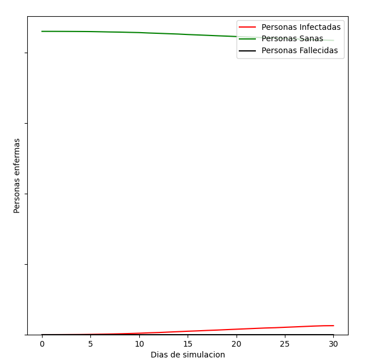
\includegraphics[width=\textwidth]{Graphics/I_M_S_43000.png}
    \caption{Datos y estimaciones de humanos infectados del modelo para 43000 personas}
    \end{minipage}\hfill
    \begin{minipage}[t]{0.5\textwidth}
    \centering
    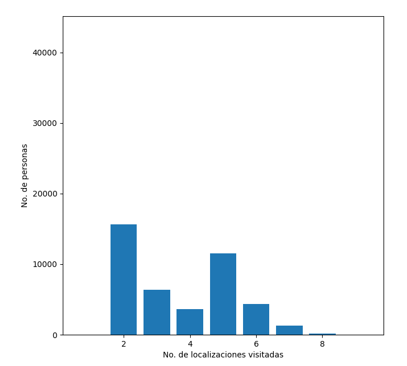
\includegraphics[width=\textwidth]{Graphics/Loc_Pers_43000.png}
    \caption{Cantidad de personas que visitaron $x$ localizaciones (43000)}
    \end{minipage}
\end{figure}
\newpage
\begin{figure}[htb]
    \centering
    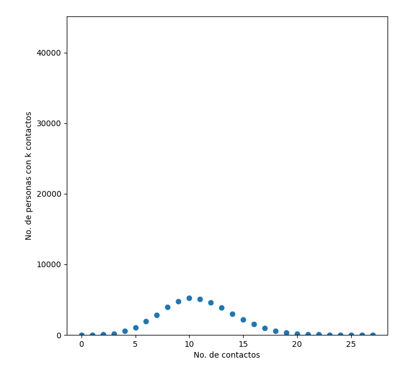
\includegraphics[width=0.5\textwidth]{Graphics/Contactos_per_43000.png}
    \caption{Cantidad de personas que visitaron $x$ localizaciones (43000)}
\end{figure}
\newpage
Este proceso tardó aproximadamente un día en ejecutarse, debido al número considerable de personas
utilizadas para el mismo. Los humanos infectados al finalizar fueron $1391$ y en los datos extraídos
de \autocite{Massón2015} da un promedio de aproximadamente $1000$ personas por mes. Ajustando los 
parámetros se puede conseguir un valor más preciso para las personas infectadas.